\documentclass[10pt,twocolumn]{article}
\usepackage[margin=0.75in]{geometry}
\usepackage{amsmath,amssymb}
\usepackage{graphicx}
\usepackage{booktabs}
\usepackage{caption}
\usepackage{subcaption}
\usepackage[hidelinks]{hyperref}
\usepackage{microtype}
\captionsetup{font=small,labelfont=bf}

\title{\vspace{-2.5em}\textbf{Deep Order-Flow Imbalance in Prediction Markets:\\
Forecasting Short-Horizon Mid-Price Returns on Polymarket}}
\author{Jing Zou\\
\small MS\&E 242: Machine Learning for Algorithmic Trading, Stanford University}
\date{\vspace{-0.8em}\small June 2026}

\begin{document}
\maketitle

\begin{abstract}
\noindent
We replicate the deep order-flow imbalance (OFI) framework of Kolm, Turiel and
Westray (2021)---originally developed on Nasdaq equity limit-order books---in a
new asset class: \emph{Polymarket binary prediction markets}. Using 2.0 million
cleaned Level-2 book snapshots from twelve NBA playoff ``series-winner''
contracts, we engineer 20-dimensional order-flow (OF) features via the Cont
three-case construction and forecast multi-horizon mid-price returns
($h=1,2,3,5,10$ ticks) with four models: a Ridge linear benchmark, a vanilla
LSTM, an LSTM-MLP, and a CNN-LSTM. Evaluated out-of-sample on a chronological
hold-out, all three neural models beat both a naive mean predictor (positive
out-of-sample $R^2$) and the linear benchmark on directional accuracy and a
frictionless Sharpe ratio. The tuned CNN-LSTM is best (directional accuracy
$\approx 62\%$, annualized Sharpe $\approx 0.63$ across seeds), but a single-layer
LSTM nearly matches it ($\approx 60\%$)---reproducing the paper's central finding
that architectural complexity adds little once OF features are used. Predictability
is concentrated at the nearest tick (directional accuracy $0.72$ at $h{=}1$ vs.\
$0.56$ at $h{=}10$), echoing that microstructure alpha lives in the immediate
next moves. The signal is small in absolute terms---expected at tick
resolution---but consistent across horizons and random seeds. We discuss
non-stationarity, the frictionless trading assumption, and the transferability of
equity-market microstructure results to prediction markets.
\end{abstract}

\section{Problem and Motivation}

\textbf{Question.} Can order-flow imbalance, the workhorse predictor of equity
market microstructure, forecast short-horizon mid-price movements in
\emph{prediction markets}? Prediction markets price the probability of a future
event (here, which NBA team wins a playoff series) as a contract that pays \$1 if
the event occurs and \$0 otherwise, so the mid-price lives in $[0,1]$ and is
literally a probability. They have a continuous limit-order book and genuine
two-sided liquidity, yet their microstructure is essentially unstudied relative to
equities.

\textbf{Target.} For each book update (``tick'') $t$ we predict the change in
mid-price $r_{t,h}=\mathrm{mid}_{t+h}-\mathrm{mid}_t$ over horizons
$h\in\{1,2,3,5,10\}$ ticks, jointly (a 5-output regression).

\textbf{Motivation.} Kolm, Turiel and Westray (2021), ``Deep Order Flow
Imbalance,'' show on Nasdaq ITCH data that (i) order-flow (OF) inputs dominate raw
order-book inputs, (ii) a simple LSTM on OF features nearly matches a far larger
CNN-LSTM, and (iii) the forecastable component decays after only a couple of price
changes. We ask whether these conclusions are \emph{intrinsic to limit-order-book
dynamics} or \emph{specific to equities}, by re-running the full pipeline on a
structurally different venue. A positive answer would establish OF imbalance as a
general microstructure signal; the economic stake is the existence of exploitable
short-horizon predictability in a fast-growing, lightly-arbitraged market.

\section{Data and Preprocessing}

\textbf{Source.} Level-2 order-book snapshots (channel
\texttt{book\_snapshot\_25}) for twelve Polymarket NBA playoff series-winner
contracts, retrieved through the Telonex API over April--May 2026 (NBA playoffs).
We keep one outcome per series. After cleaning, the corpus contains
\textbf{2{,}041{,}832 snapshots}; per-market depth ranges from 39k (Suns vs.\
Thunder) to 403k (Lakers vs.\ Rockets) valid rows.

\textbf{Cleaning.} Snapshots are time-sorted; $\sim$7--10\% exact/near-simultaneous
duplicates are collapsed to the last book state per microsecond; rows with a
missing best level or an inverted book ($\mathrm{bid}_0\!\ge\!\mathrm{ask}_0$,
$0.03$--$0.63\%$ per market) are dropped; the mid is
$(\mathrm{bid}_0+\mathrm{ask}_0)/2$. Deeper missing levels are filled to be
numerically consistent with the OF construction: missing bid price $\to 0$
(probability lower bound), missing ask price $\to 1$ (upper bound), missing size
$\to 0$ (no resting order).

\textbf{Order-flow features.} Following Cont et al.\ and Kolm et al., we compute a
signed order-flow value per level that isolates the \emph{change} in resting
liquidity. For bid level $i$ with price $b^i_t$ and size $v^{i,b}_t$:
\begin{equation}
\mathrm{bOF}^i_t=
\begin{cases}
+\,v^{i,b}_t & b^i_t > b^i_{t-1}\ \text{(new bid)}\\
\;\;v^{i,b}_t-v^{i,b}_{t-1} & b^i_t = b^i_{t-1}\ \text{(size change)}\\
-\,v^{i,b}_t & b^i_t < b^i_{t-1}\ \text{(bid pulled)}
\end{cases}
\end{equation}
with the signs mirrored on the ask side (a rising ask removes liquidity, so
$\mathrm{aOF}$ takes the opposite sign convention). Concatenating $10$ bid and $10$
ask levels gives an $\mathrm{OF}_t\in\mathbb{R}^{20}$ vector per tick. Each model
input is a look-back window of $W{=}100$ ticks, shape $(100,20)$; windows never
cross market boundaries.

\textbf{Normalization.} OF features are heavy-tailed (large orders create extreme
outliers atop a spike at zero; Fig.~\ref{fig:ofdist}, left). We winsorize each
feature at its $[0.5\%, 99.5\%]$ \emph{training} quantiles, then $z$-score with
training mean/variance, yielding a compact, zero-centered, unit-variance input
(Fig.~\ref{fig:ofdist}, right) well-suited to neural sequence models. Prediction
targets are likewise $z$-scored with training statistics, so a mean predictor
attains a standardized MSE of exactly $1.0$---a convenient ``did the model learn
anything?'' threshold.

\textbf{Splits.} Each market is split \emph{chronologically} into validation
(earliest 15\%), training (next 70\%), and test (latest 15\%); this keeps the test
set the most recent data and avoids look-ahead. Windows are then formed at every
$s$-th valid tick ($s$ is the \emph{stride}, a tuned data-volume lever). With
evaluation stride $10$ the held-out sets contain $30.5$k validation and $30.6$k
test windows; training windows range from $57$k (stride 25) to $143$k (stride 10).

\begin{figure}[t]
\centering
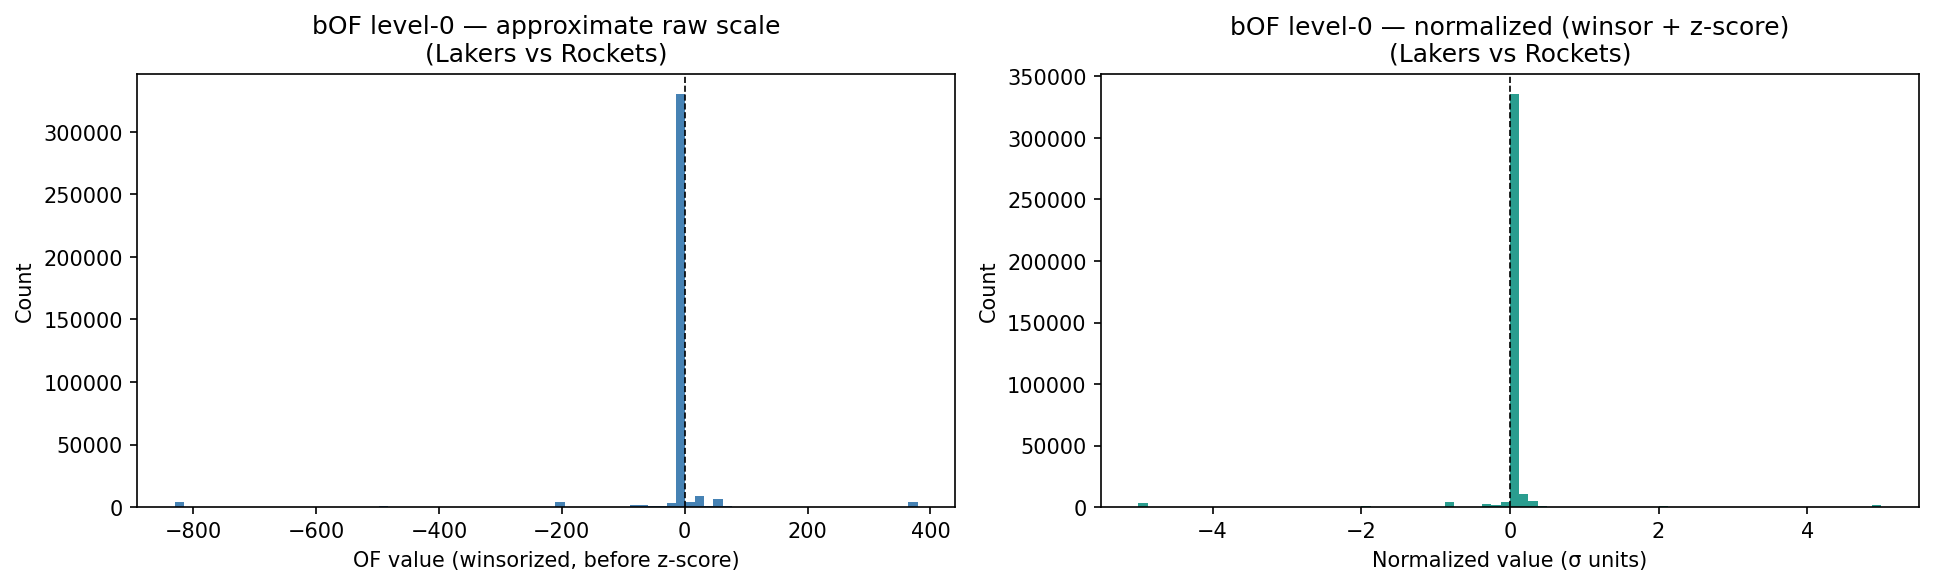
\includegraphics[width=\linewidth]{results/viz_05_of_distribution.png}
\caption{Order-flow feature distribution for the largest market, raw
(post-winsorization, heavy-tailed with a zero spike) vs.\ normalized (compact,
$\approx\!\mathcal{N}(0,1)$). Normalization is essential for stable training.}
\label{fig:ofdist}
\end{figure}

\section{Exploratory Data Analysis}

Three properties of the data shape the modeling choices.

\textbf{(1) Liquidity is real but heterogeneous.} Median spreads range
$0.007$--$0.020$ (probability units); the fraction of snapshots with spread
$<0.05$ (``tight'') ranges $0.69$--$0.999$. All twelve contracts clear a 60\%
tight-fraction usability bar, so every book is genuinely two-sided
(Table~\ref{tab:data}). Mid-prices span the unit interval (median mids from
$0.01$ to $0.96$), i.e.\ we include both near-certain and toss-up markets.

\textbf{(2) Returns are sparsely non-zero, and more so at longer horizons.} Most
ticks do not move the mid: the non-zero fraction rises from $11\%$ at $h{=}1$ to
$34\%$ at $h{=}10$ (Table~\ref{tab:nonzero}). This zero-inflation is why we score
directional accuracy only on ticks that actually moved (Sec.~\ref{sec:metrics});
scoring flat ticks would merely reward predicting zero.

\textbf{(3) Time is event-driven.} Snapshots arrive irregularly (median
inter-snapshot gap $\sim$0.05--0.3\,s), so we model in \emph{tick time}, not
clock time---consistent with the OF construction, which is defined per book
update.

\begin{table}[t]
\centering\small
\caption{Market summary across the twelve NBA contracts (aggregate).}
\label{tab:data}
\begin{tabular}{lc}
\toprule
Quantity & Value / range \\
\midrule
Contracts (all usable)            & 12 \\
Cleaned snapshots (total)         & 2{,}041{,}832 \\
Valid rows per market             & 39k -- 403k \\
Median spread                     & 0.007 -- 0.020 \\
Tight-spread fraction ($<0.05$)   & 0.69 -- 0.999 \\
Median mid-price                  & 0.011 -- 0.960 \\
LOB depth used (bid+ask)          & 10 + 10 levels \\
\bottomrule
\end{tabular}
\end{table}

\begin{table}[t]
\centering\small
\caption{Fraction of ticks with a non-zero mid-price change, by horizon
(pooled). Predictability and sample coverage both grow with $h$.}
\label{tab:nonzero}
\begin{tabular}{lccccc}
\toprule
Horizon $h$ (ticks) & 1 & 2 & 3 & 5 & 10 \\
\midrule
Non-zero fraction & 0.11 & 0.18 & 0.23 & 0.29 & 0.34 \\
\bottomrule
\end{tabular}
\end{table}

\section{Models}

All models map a $(100,20)$ OF window to five horizon returns. They share data,
loss, and evaluation; only the function class differs.

\textbf{Ridge (linear benchmark).} The window is flattened to $2000$ dimensions
and regressed on the five targets with Ridge ($\alpha{=}1$), fit on up to $40$k
training windows. This is our ``reasonable benchmark'' and a proxy for the paper's
linear AR-X baseline.

\textbf{LSTM.} A single-layer LSTM (hidden $128$) consumes the window; its last
hidden state feeds a linear read-out to five horizons. The forget-gate bias is
initialized to $1.0$ (Gers et al.) to ease gradient flow. $\approx$77k parameters.

\textbf{LSTM-MLP.} Identical trunk, but the linear read-out is replaced by a small
MLP head ($1$ hidden layer of $64$, ReLU). A strict generalization of the LSTM
(the head collapses to the linear read-out when the hidden layer is removed).
$\approx$85k parameters.

\textbf{CNN-LSTM.} The paper's strongest model: stacked 1-D convolution blocks
over the OF sequence, an Inception module (parallel multi-scale filters), then an
LSTM (hidden $64$) and a linear read-out. The convolutions act as a learned local
feature extractor before the recurrent layer. $125{,}125$ parameters.

\section{Training, Validation, and Testing}

Models are trained by minimizing mean-squared error on the standardized targets
with Adam, gradient clipping (max-norm $1.0$), batch size $256$, and up to
$60$ epochs with early stopping (patience $8$) on the \emph{validation} loss; the
best-validation weights are restored before testing. The test set is touched
\emph{once}, for the final reported numbers. Predictions are un-standardized to raw
return units before all metrics. Compute ran on cloud GPUs (Modal; T4--H100). To
prevent look-ahead, all normalization statistics (winsor bounds, OF and target
mean/variance) are estimated on the training split only and frozen for
validation/test.

\section{Hyperparameter Selection}

We tune in three stages, always selecting on validation loss, never on test
metrics, and varying one axis per stage. \textbf{Stage 1} sweeps the learning rate
and the training stride (data volume); \textbf{Stage 2} sweeps capacity (LSTM
width/depth, and the MLP head for LSTM-MLP); \textbf{Stage 3} re-runs finalists
across random seeds for a stability estimate. The CNN-LSTM was tuned through all
three stages (18 runs); the LSTM and LSTM-MLP are reported from their Stage-1 best
configuration.

A clear, reproducible \emph{under-training} pathology emerged: the paper's Nasdaq
learning rate ($10^{-5}$) is far too small here---train loss fell only
$1.004\!\to\!0.989$ over 50 epochs and never early-stopped, i.e.\ the model barely
beat the mean predictor. Raising the learning rate to $10^{-3}$--$2\!\times\!10^{-3}$
(CNN-LSTM) and increasing data volume via stride-10 windows fixed it. The final
CNN-LSTM uses lr $2\!\times\!10^{-3}$, stride $10$, hidden $64$, no weight decay
(regularization did not help, consistent with the train/test gap being
distribution shift rather than over-fitting).

\section{Performance Evaluation}
\label{sec:metrics}

We report three complementary metrics, each computed per horizon and averaged,
in-sample and out-of-sample, against the naive train-mean predictor.

\textbf{(1) Out-of-sample $R^2$.} Variance explained relative to the naive
constant-mean predictor:
\begin{equation}
R^2_{\mathrm{OS}} = 1 - \frac{\sum (\hat r - r)^2}{\sum (\bar r_{\text{train}} - r)^2}.
\end{equation}
$>0$ means the model beats ``always predict the average.'' At tick resolution,
signal-to-noise is tiny, so values of $10^{-3}$--$10^{-2}$ already indicate a real
edge; $0.5$ would signal leakage.

\textbf{(2) Directional accuracy.} The rate at which $\mathrm{sign}(\hat r)$
matches $\mathrm{sign}(r)$, computed only on moved ticks ($r\neq 0$). Baseline
$0.50$.

\textbf{(3) Annualized Sharpe.} A frictionless strategy takes a unit position in
the predicted direction; with $\mathrm{pnl}_t=\mathrm{sign}(\hat r_t)\,r_t$,
$\text{Sharpe}=\mathrm{mean}(\mathrm{pnl})/\mathrm{std}(\mathrm{pnl})\times\sqrt{252}$.
We additionally persist the full per-tick PnL series (mean PnL, win rate, and
max drawdown) for the out-of-sample set.

\section{Results}

\begin{table*}[t]
\centering\small
\caption{Out-of-sample performance (mean over the five horizons). All neural OF
models beat both the naive predictor ($R^2_{\mathrm{OS}}>0$) and the Ridge linear
benchmark on every metric. CNN-LSTM is best; the single-layer LSTM nearly matches
it. CNN-LSTM is tuned through 3 stages and seed-averaged; LSTM/LSTM-MLP are
single-seed Stage-1 bests. Higher is better for all three metrics.}
\label{tab:main}
\begin{tabular}{lrrrl}
\toprule
Model & $R^2_{\mathrm{OS}}$ (mean) & Directional acc. & Sharpe (ann.) & Notes \\
\midrule
Naive (train-mean)        & $0.0000$  & $0.500$ & $0.000$ & by construction \\
Ridge linear benchmark    & $-0.0110$ & $0.562$ & $0.130$ & overfits; loses to naive on $R^2$ \\
LSTM (single layer)       & $+0.0004$ & $0.604$ & $0.412$ & $\approx$77k params \\
LSTM-MLP                  & $+0.0003$ & $0.598$ & $0.399$ & $\approx$85k params \\
\textbf{CNN-LSTM (tuned)} & $\mathbf{+0.0020}$ & $\mathbf{0.620}$ & $\mathbf{0.569}$ & seed-avg: $+0.0031$, $0.622$, $0.631$ \\
\bottomrule
\end{tabular}
\end{table*}

\textbf{The OF signal is real and beats both baselines.} Table~\ref{tab:main}
summarizes out-of-sample performance. Every neural model attains a
\emph{positive} $R^2_{\mathrm{OS}}$ (it beats the naive mean predictor), whereas
the Ridge benchmark is \emph{negative} ($-0.011$): the linear model over-fits the
2000-dimensional flattened window and loses to naive out-of-sample. On directional
accuracy the neural models reach $0.60$--$0.62$ versus $0.562$ for Ridge and
$0.50$ for chance; on Sharpe, $0.40$--$0.57$ versus $0.13$ for Ridge.

\textbf{Architectural complexity adds little.} The tuned CNN-LSTM is best
(directional accuracy $0.620$, Sharpe $0.569$; seed-averaged $0.622\pm0.007$ and
$0.631\pm0.039$ across three seeds, with $R^2_{\mathrm{OS}}=0.0031\pm0.0010$), but
a single-layer LSTM with $1.7\times$ fewer parameters reaches $0.604$ directional
accuracy---and the LSTM-MLP head buys nothing over the plain LSTM. This directly
reproduces the paper's headline conclusion that, \emph{once OF features are used},
a simple recurrent model captures most of the available signal.

\textbf{The nearest tick is the most predictable.} For the CNN-LSTM, directional
accuracy is highest at $h{=}1$ ($0.719$) and lowest at $h{=}10$ ($0.561$), with a
non-monotonic dip in between ($0.597$--$0.626$ at $h{=}2,3,5$;
Table~\ref{tab:horizon}, Fig.~\ref{fig:results}). The immediate next move is by far
the most forecastable from recent order flow---the prediction-market echo of the
paper's ``alpha decays after a couple of price changes.'' Sharpe, by contrast,
shows \emph{no} clean horizon trend (range $0.48$--$0.67$, in fact lowest at
$h{=}1$ and $h{=}5$): because a unit position is taken on every tick, Sharpe mixes
directional skill with the per-horizon return scale and is the noisiest of the
three metrics, so we read the horizon structure off directional accuracy rather
than Sharpe.

\textbf{In- vs.\ out-of-sample.} In-sample directional accuracy ($\approx0.62$) is
only modestly above out-of-sample, and both are positive on every horizon,
indicating the signal is genuine rather than memorized. The large
\emph{loss-scale} gap (standardized validation MSE $\approx 3.5$ vs.\ training
$\approx 0.9$) is not classic over-fitting---weight decay did not help---but
reflects non-stationarity: the held-out period is intrinsically more volatile than
the training period (Sec.~\ref{sec:limits}).

\begin{table}[t]
\centering\small
\caption{CNN-LSTM out-of-sample metrics by horizon (seed 42). Predictability is
concentrated at the nearest tick and decays with $h$.}
\label{tab:horizon}
\begin{tabular}{lccccc}
\toprule
Horizon $h$        & 1 & 2 & 3 & 5 & 10 \\
\midrule
$R^2_{\mathrm{OS}}$       & 0.0007 & 0.0031 & 0.0018 & 0.0011 & 0.0031 \\
Directional acc.   & 0.719 & 0.597 & 0.626 & 0.597 & 0.561 \\
Sharpe (ann.)      & 0.476 & 0.608 & 0.666 & 0.476 & 0.620 \\
\bottomrule
\end{tabular}
\end{table}

\begin{figure}[t]
\centering
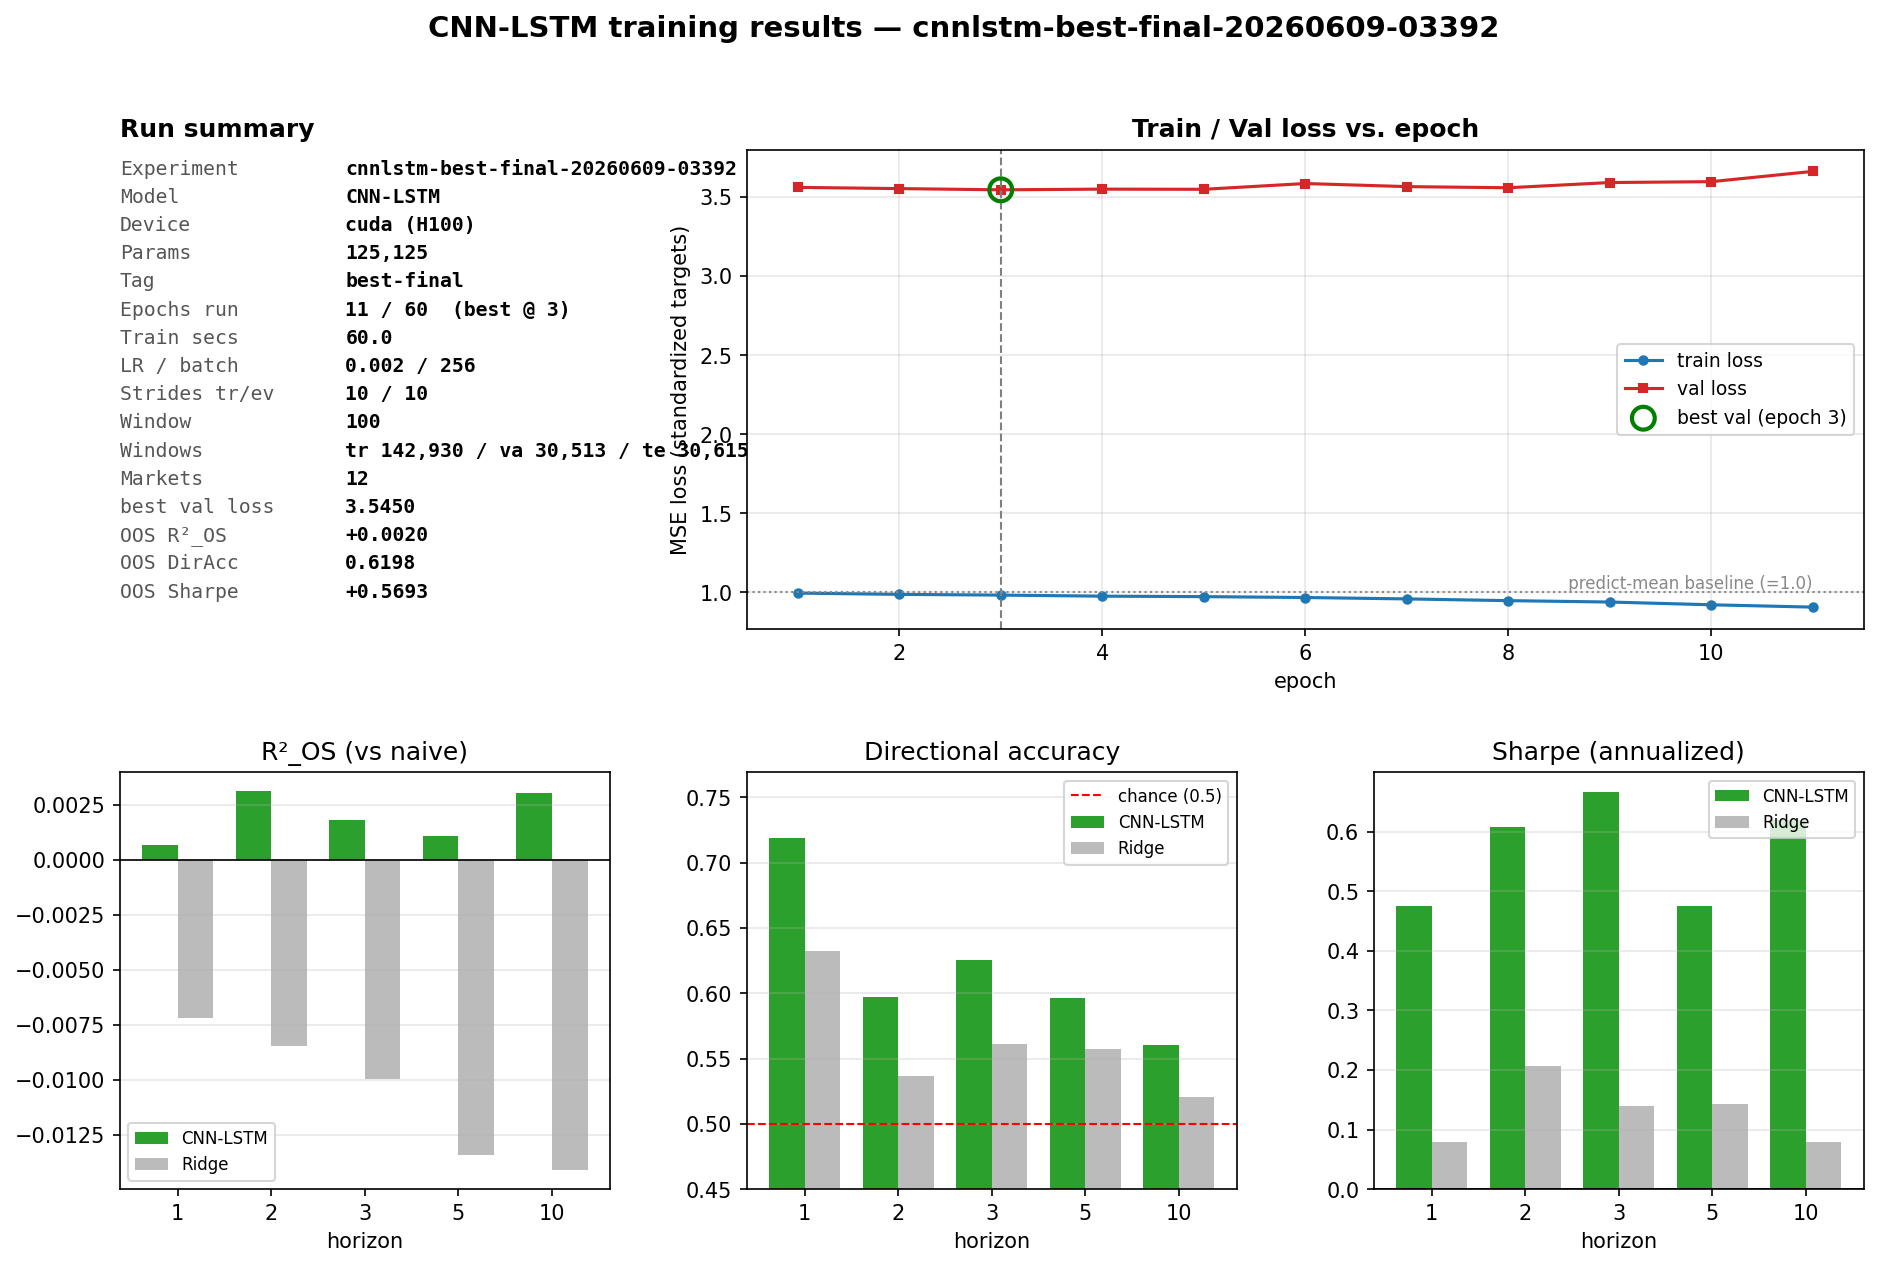
\includegraphics[width=\linewidth]{results/viz_07_results_best-final.png}
\caption{Tuned CNN-LSTM: training/validation loss (left) and per-horizon
out-of-sample metrics (right). Validation loss bottoms early (epoch 3) and early
stopping restores those weights; directional accuracy and Sharpe decay with
horizon.}
\label{fig:results}
\end{figure}

\section{Discussion and Interpretation}

The economic reading is that order-flow imbalance carries genuine, exploitable
information about the next few mid-price moves in Polymarket NBA contracts---the
same signal documented in equities, now shown to transfer to a market that prices
probabilities rather than dollars. The magnitude is small ($R^2$ near $10^{-3}$),
which is exactly what microstructure theory predicts at tick resolution: most of
the variance is unpredictable noise, and a thin but persistent drift is
forecastable from recent liquidity changes. A $\sim$62\% directional hit rate at
$h{=}1$ with positive risk-adjusted expectancy is meaningful evidence of a tradable
micro-edge, while the rapid horizon decay tells us any such edge must be harvested
almost immediately. That a single-layer LSTM essentially ties the CNN-LSTM is the
practically important message: the value is in the \emph{feature representation}
(signed order flow), not in deep architecture---so the cheaper model is the
sensible production choice.

\section{Limitations and Conclusion}
\label{sec:limits}

\textbf{Limitations.} (1) \emph{Non-stationarity.} The standardized
train/validation loss gap ($\sim$0.9 vs.\ $\sim$3.5) shows the hold-out period is
materially more volatile than training; metrics are conditional on this regime, and
selecting on a validation block drawn from the earliest data may not reflect the
test regime. (2) \emph{Frictionless PnL.} The Sharpe ignores fees, slippage, and
the wide prediction-market spreads ($0.007$--$0.020$); a strategy that flips every
tick would not survive realistic costs, so Sharpe is a signal-quality readout, not
a backtest. (3) \emph{Pooled, not per-stock.} Unlike the paper's per-instrument
models, we pool all twelve contracts into one model (limited per-market data);
this trades faithfulness for sample size. (4) \emph{Scope.} Twelve NBA series over
one playoff window is a narrow sample; single-seed Stage-1 results for the LSTM
models carry seed noise. (5) \emph{Tick time.} Event-driven sampling means a
``tick'' is not a fixed time interval, complicating clock-time interpretation.

\textbf{Conclusion.} Replicating Deep Order Flow Imbalance on Polymarket
prediction markets, we find its core results transfer: OF features plus a modest
recurrent model forecast short-horizon mid-price returns with positive
out-of-sample $R^2$, $\sim$60--62\% directional accuracy, and a positive
frictionless Sharpe, beating both a naive and a linear benchmark; a simple LSTM
nearly matches the CNN-LSTM; and predictability is concentrated in the nearest
ticks. The edge is small but consistent across horizons and seeds. The main open
problems are cost-aware evaluation and handling the non-stationarity that
dominates the loss scale---both essential before any of this becomes a strategy.

\section*{Acknowledgments}
\textbf{Data:} Polymarket order books via the Telonex API. \textbf{Software:}
PyTorch, scikit-learn, NumPy, pandas; cloud GPUs via Modal. \textbf{AI tools:}
Anthropic Claude (Claude Code) was used to help implement the training/evaluation
code, hyperparameter-sweep scripts, and to assist in drafting this report; all
modeling decisions, results, and interpretations are the author's. \textbf{Method:}
this work replicates Kolm, Turiel \& Westray (2021).

\begin{thebibliography}{9}
\small
\bibitem{kolm} P.~N. Kolm, J.~Turiel, and N.~Westray. ``Deep Order Flow
Imbalance: Extracting Alpha at Multiple Horizons from the Limit Order Book.''
\emph{Mathematical Finance}, 2023 (preprint 2021).
\bibitem{cont} R.~Cont, A.~Kukanov, and S.~Stoikov. ``The Price Impact of Order
Book Events.'' \emph{Journal of Financial Econometrics}, 12(1), 2014.
\bibitem{gers} F.~A. Gers, J.~Schmidhuber, and F.~Cummins. ``Learning to Forget:
Continual Prediction with LSTM.'' \emph{Neural Computation}, 12(10), 2000.
\bibitem{zhang} Z.~Zhang, S.~Zohren, and S.~Roberts. ``DeepLOB: Deep Convolutional
Neural Networks for Limit Order Books.'' \emph{IEEE Trans. Signal Processing},
67(11), 2019.
\end{thebibliography}

\end{document}
